\chapter{Discussion}

\section{Initialization Matters}

During multiple hyperparameter searches performed, an interesting phenomenon emerged. If the initial neuron positions and orientations are far from the truth and if the initial standard deviation of the Gaussian distribution is too large, the network does not converge. The network usually converges and performs well if the initial neural positions and orientations are in the range of $[-0.7, 0.7]$ or smaller with a standard deviation below approximately 0.5. Moreover, networks with the same architectures and hyperparameters trained with a different seed (and, therefore, different initial positions and orientations of the neurons) were significantly inconsistent in their performance (Figure~\ref{initialization_matters}). The motives behind such high-performance variability are likely to be connected to the initialization of the readout parameters. Further research aimed at better identifying such motives could be performed in the future and possibly produce more consistently optimal performances.

\begin{figure}[H]\centering
	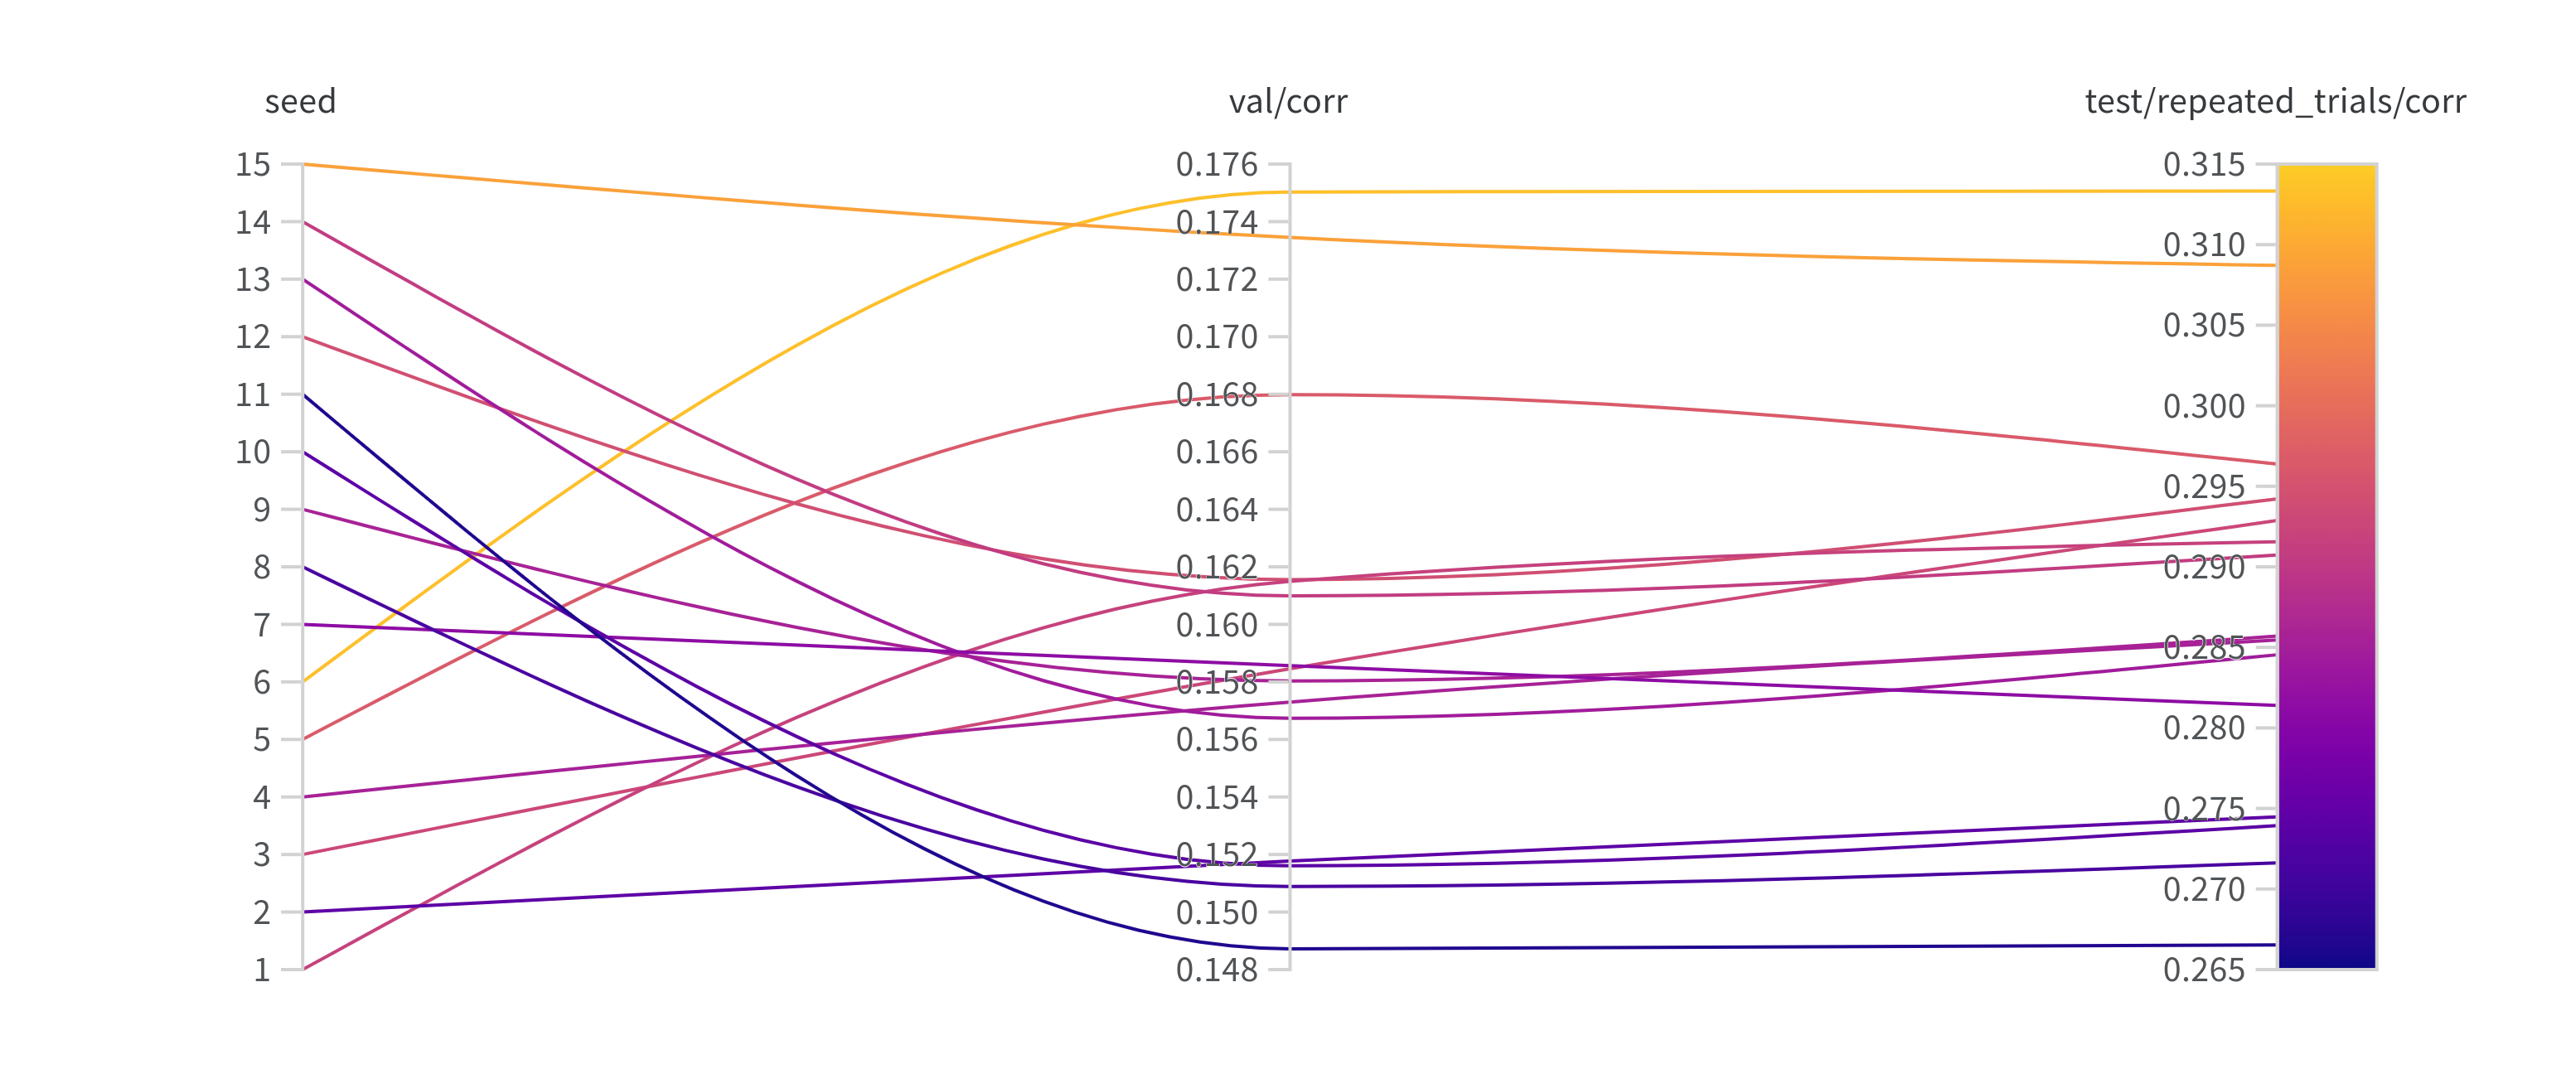
\includegraphics[width=150mm]{../img/initialization_matters.png}
	\caption{This figure represents the results of one of the best-performing network architectures trained on the mouse dataset with the number of orientations set to 24. The hyperparameters are shared between all seeds. Each line represents a result of a model with a particular seed. Clearly, initialization significantly influences the network’s performance.}
	\label{initialization_matters}
\end{figure}

\section{Different Datasets Yield Different Results}\label{diff_results}

The models exhibited interesting differences when comparing the results obtained from the two different datasets.

The correlation fraction with respect to the control model achieved on the synthetic dataset was higher than the one obtained with the experimental dataset. This result is, however, expected. Although Antolík's model \citep{antolik2019comprehensive} is a very accurate model of a cat V1, being a model, it still makes simplifying abstractions regarding specific details of the V1 visual information encoding. One example of such simplification is, for instance, the absence of direction selectivity. Another example, for instance, is the absence of other brain areas that are known to influence V1 activity in biological systems. For this reason, the in-silico model is likely to perform a simpler information encoding and present a lower degree of intrinsic noise than the experimental dataset from Lurz et al. \citep{lurz2021generalization}. As a consequence, the performance drop with respect to the control model was lower in the dataset generated by the computational model.


\section{Lack of Computational Resources}

We would likely be able to achieve even higher prediction performance with more computational power. The computation time on MetaCentrum machines with GPU is limited to a maximum length of 24 hours. This was a limiting factor for networks trained on the synthetic dataset, leading to under-fitted models, sometimes misleading the Bayesian search into hyperparameter subspaces with non-optimal hyperparameters. Moreover, if more sweeps were performed, gradually narrowing the hyperparameters space, we would probably be able to find hyperparameters that would conceive even better models. 

Despite the lack of computational resources, we designed and trained deep neural networks that achieve a very high performance relative to the control model based on the state-of-the-art models for predicting neural responses. Specifically, the best model trained on the synthetic dataset generated by Antolík et al. model \citep{antolik2019comprehensive} achieved a 0.8327 correlation fraction with respect to the control model. In contrast, the best model trained on the experimental dataset from Lurz et al. \citep{lurz2021generalization} achieved 0.6651 of the same measure. While the control architecture predicts a neuron's response based on a whole vector of features, our model is restrained to using just a scalar value from the reCNN core. This bottleneck reduces the predictive performance. Based on the results, the bottleneck influenced models trained on the mouse dataset more than the models trained on the in-silico dataset, as discussed in the previous section.

\section{Reconstruction of orientation map of the Antolík et al. model}

Due to the surprisingly accurate estimates of the neural locations and their preferred orientations, we reconstructed the orientation map of the Antolík et al. model \citep{antolik2019comprehensive}. Moreover, we examined important statistics of this reconstruction. Namely, the average error of the location estimate was 0.1 degrees of visual angle, while the average error of the preferred orientation estimate was 15.93 degrees \footnote{Note that the units are different!}.

Interestingly, in the distribution of errors of position estimates, a small portion of neurons ($0.16 \%$) exhibited a significantly larger error than the remaining neurons' estimates. In future work, it would be interesting to investigate the cause of this problem.

Although the reconstructed orientation map was very accurate, being it not our primary objective, we did not optimize our network to predict the neural locations and preferred orientations. If we had done so, the resulting orientation map might have been of even higher quality. Therefore, we propose to use our approach and slightly alter the network's behavior to focus not on the predictive neural response performance but on the accuracy of the location and preferred orientation estimates. This could be achieved by constraining the kernel sizes in the reCNN core in such a way that we obtain features in the bottleneck layer with a receptive area spanning the same degree of visual angle as the receptive field of the actual neurons in V1 of the species on which the data was obtained. This way, we might be able to model the primary visual cortex more plausibly with regard to the characteristics of certain species. Consequently, the architecture might estimate the neurons’ positions and orientation preferences with higher precision.

As regards the higher error in prediction of the preferred orientation, it might have been caused by a lower orientation selectivity of a certain neuron. If the particular neuron is not very orientation selective, it is unclear what the exact orientation preference is; therefore, the predicted preference is inaccurate.

\section{Hyperparameters of the Best Models}

The best networks tend to prefer relatively large kernels (the best models on both datasets had all kernels of sizes larger than 10). It would be interesting to investigate how large the area of interest of the final bottleneck layer is and compare it to the size of the receptive field of real neurons in the primary visual cortex of a mouse or a cat.

Both models chose the learning rate of 0.001 and a small number of channels (4 and 8, respectively). The fewer channels were likely to be caused by the number of orientations that linearly increase the number of core parameters, leading to a higher learning capacity sufficient to learn all necessary patterns in the training dataset.


